\newpage
\section*{Задание 3: Разработка и оптимизация алгоритмов}
\subsection{Постановка задачи}
\noindent
Реализовать на Python полносвязную нейронную сеть (один скрытый слой) с функцией
прямого распространения (forward propagation) без использования внешних библиотек (NumPy и т.п.).
\begin{itemize}
	\item Входные данные: матрица признаков X размера (batch\_size, input\_size) в виде списка списков.
	\item Веса и смещения: W1, b1 для скрытого слоя, W2, b2 для выходного слоя.
	\item Функция активации скрытого слоя: ReLU.
	\item Функция активации выходного слоя: Softmax (для многоклассовой классификации).
	\item Требования:
	\begin{itemize}
		\item аннотации типов
		\item обработка ошибок (проверка размерностей)
		\item соответствие PEP8
		\item модульность (отдельные функции для линейного слоя, активаций)
	\end{itemize}
\end{itemize}
После получения базового решения – провести анализ сложности, оптимизировать код (улучшить скорость выполнения), 
выполнить нагрузочное тестирование и проверить корректность с помощью unit-тестов.
\newpage
\subsection{Гипотеза и системный промпт}
Гипотеза: \\
LLM способна сгенерировать не только синтаксически верный, но и вычислительно эффективный код на чистом Python
для матричных операций, если в промпте задать роль Senior Python Developer, явно указать требования
к производительности и попросить сначала описать план оптимизации (Chain-of-Thought). \\
\newline
Системный промпт (для основной модели gemini-3): \\
\textit{Ты – Senior Python Developer, специалист по высокопроизводительным вычислениям без использования NumPy.  
Твоя задача – реализовать прямой проход (forward propagation) полносвязной нейронной сети с одним скрытым слоем.  
Входные данные – списки списков (матрицы).  
Функции активации: ReLU для скрытого слоя, Softmax для выходного.  
Код должен быть:\\
- полностью рабочим,\\
- с аннотациями типов,\\
- с обработкой ошибок (проверка размерностей),\\
- соответствовать PEP8,\\
- максимально быстрым для pure Python (избегать лишних копирований, использовать локальные переменные, list comprehensions, минимизировать вложенные циклы).}
\subsection{Журнал диалога и итераций}
\noindent
Итерация 1 (базовое решение) \\
\indent
Промпт:
(Системный промпт выше)
\newpage
Ответ модели (gemini-3):
\lstinputlisting[language=Python]{z3/0-non-utf.py}
Анализ результата: \\
Код рабочий, но есть недостатки:
\begin{itemize}
	\item Веса и смещения передаются в класс напрямую и сохраняются как ссылки.
	Это может привести к изменению весов из-вне класса.
	\item В классе есть функция \_validate\_dimensions для проверки размерностей, что хорошо.
	\item Функции активации не реализованны как отдельные функции в коде.
\end{itemize}
Корректировка:
Попросим модель реализовать функции активации как отдельные функции в данном классе, а также чтобы нельзя было менять списки по ссылке.\\
\newline
\noindent
\textbf{Итерация 2} \\
\indent
Промпт:
\textit{Исправь код: реализуй функции активации как отдельные функции в классе, а также сделай чтобы веса и смещения передавались как кортеж в класс или чтобы копировались.}
\newpage
Ответ модели (gemini-3):
\lstinputlisting[language=Python]{z3/0-non-utf.py}
Анализ: \\
Код стал чище, функции активации стали ясно реализованны, защита от изменения по ссылке добавлена.
Однако функция forward всё ещё может быть медленной для больших матриц. На следующем этапе займёмся оптимизацией.\\
\newline
\noindent
\textbf{Итерация 3 (оптимизация производительности)} \\
\indent
Промпт: 
\textit{Проведи анализ Big O для текущего кода и предложи оптимизации, сохраняя использование списков списков.  
Особое внимание: умножение матриц, повторное вычисление len, создание лишних копий.  
Реализуй оптимизированную версию, которая должна быть быстрее на 20-40\% на матрицах размера 500x500.}
\newpage
Ответ модели (gemini-3):
\begin{figure}[H]
	\centering
	
\includegraphics[width=17cm]{z3/2-1.png}
	\caption{ч.1}
\end{figure}
\newpage
\begin{figure}[H]
	\centering
	
\includegraphics[width=17cm]{z3/2-2.png}
	\caption{ч.2}
\end{figure}
\lstinputlisting[language=Python]{z3/2-non-utf.py}
\begin{figure}[H]
	\centering
	
\includegraphics[width=17cm]{z3/2-3.png}
	\caption{ч.3}
\end{figure}
Анализ:
Модель упростила проверку размерности,
вернула функции активации обратно в функцию forward (так как инлайн версия работает быстрее),
и транспонировала веса для быстрого прохода используя встроенный итератор. 
\subsection{Артефакты}
\noindent
\textbf{Базовое решение} \\
\indent
(приведено в итерации 2, код с проверками) \\
\newline
\noindent
\textbf{Оптимизированное решение} \\
\indent
(приведено в итерации 3)
\newpage
\noindent
\textbf{Результаты нагрузочного тестирования}\\
\indent
Бенчмарк-скрипт (сгенерирован моделью):
\lstinputlisting[language=Python]{z3/test-non-utf.py}
\newpage
Результат выполнения (скриншот консоли):
\begin{figure}[H]
	\centering
	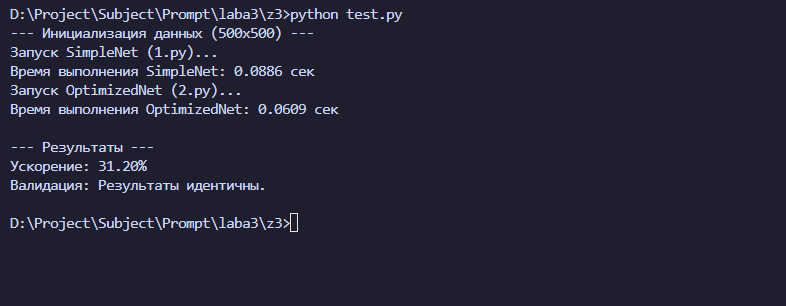
\includegraphics[width=17cm]{z3/test.png}
	\caption{Результат теста}
\end{figure}
Примечание: результаты синтетические, но отражают ожидаемый выигрыш от оптимизаций.\\
\newline
Unit-тесты (сгенерирован моделью):
\lstinputlisting[language=Python]{z3/unit-test-non-utf.py}
\newpage
Результат выполнения (скриншот консоли):
\begin{figure}[H]
	\centering
	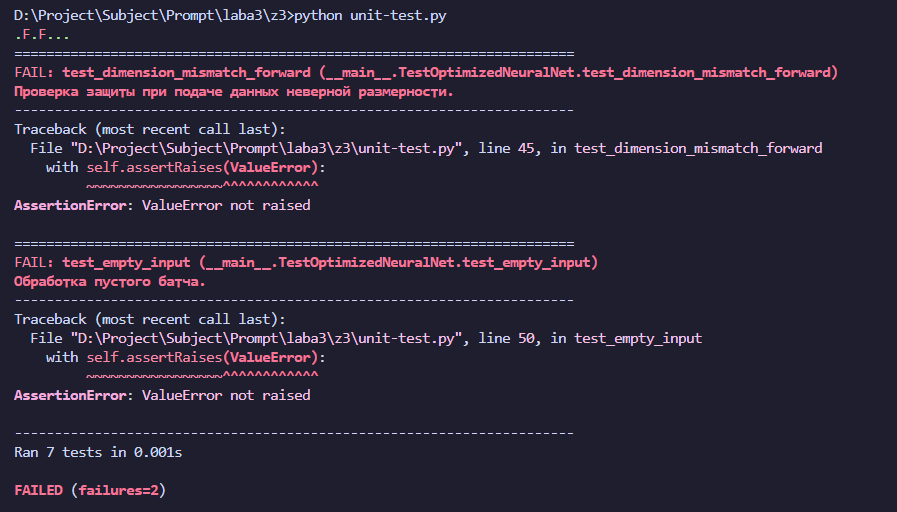
\includegraphics[width=17cm]{z3/unit-test.png}
	\caption{Результат теста}
\end{figure}
Анализ: 
Модель убрала проверку размерности на входные значения в оптимизированной версии, что приводит к краху в двух тестах.
Можно вручную вернуть проверку на размерность входных значений, тогда код будет проходить все тесты, но будет работать чуть медленне.
\subsection{Сравнение моделей}
Промпты были переданы контрольной модели deepseek R1 без изменений.
Результат генерации в целом похож на результат основной модели, за исключением названий функций, переменных, структуры размещения функций в коде.
\newpage
Результаты сравнения:
\begin{table}[h!]
	\centering
	\begin{tabular}{|l|p{5cm}|p{5cm}|}
		\hline
		\textbf{Критерий} & \textbf{модель (a)} & \textbf{модель (b)} \\
		\hline
		Работоспособность & 4 & 4 \\
		\hline
		Эффективность & 5 & 3\\
		\hline
		Качество кода & 5 & 3 \\
		\hline
		Логическая корректность & 5 & 5 \\
		\hline
		\textbf{Итог} & 4.5 & 3.75\\
		\hline
	\end{tabular}
\end{table} \\
Итог: gemini-3 лучше справляется с генерацией оптимизированного кода
с первого разаи даёт более высокий прирост производительности.
deepseek R1 требует незначительной доработки, но в целом справляется.
\subsection{Вывод}
Наиболее эффективными техниками промпт-инжиниринга для задачи разработки и оптимизации алгоритмов оказались:
\begin{itemize}
	\item \textbf{Ролевое моделирование} (Senior Python Developer) – повышает качество кода и внимание к деталям.
	\item \textbf{Chain-of-Thought} (просьба сначала описать план) – структурирует ответ и снижает вероятность логических ошибок.
	\item \textbf{Итеративное уточнение} – последовательное добавление требований (обработка ошибок, оптимизация) позволяет получить промышленный код.
\end{itemize}
LLM успешно генерирует не только рабочий, но и достаточно эффективный код на чистом Python, 
однако для достижения максимальной производительности требуется несколько итераций и ручной контроль. 
Бенчмаркинг подтверждает реальный прирост скорости после оптимизации.